\documentclass{beamer}
\mode<presentation>{}

\graphicspath{ {./figures/} }
\usepackage{enumitem,xcolor}
\usepackage{tikz}
\usetikzlibrary{shadows,arrows.meta,positioning,backgrounds,fit}
\usepackage{subcaption}
\usepackage{natbib}     %% for bibliography
\bibliographystyle{plainnat}

%\setbeamertemplate{footline}[frame number]
%\setbeamertemplate{headline}{}
\setbeamertemplate
 {footline}{\quad\hfill\insertframenumber/\inserttotalframenumber\strut\quad}

% colored underline, with Beamer overlay support
% usage: \cul{x} or \cul[blue]{x} or \cul<2->{x} or \cul<2->[blue]{x}
\newcommand<>{\cul}[2][red]{%
  % change underline dimentions: https://tex.stackexchange.com/a/167957/25264
  \fontdimen8\textfont3=0.75pt%
  % colored underline: https://tex.stackexchange.com/a/9477/25264
  % transparent underline: https://tex.stackexchange.com/a/45601/25264
  % switch between colored and transparent: http://mirrors.ibiblio.org/CTAN/macros/latex/contrib/beamer/doc/beameruserguide.pdf sections 9.3 and 9.6.1
  \alt#3%
      {\color{#1}\underline{{\color{black}#2}}\color{black}}%
      {\transparent{0.0}\underline{{\transparent{1.0}#2}}\transparent{1.0}}%
}

% so that the captions are numerated
\setbeamertemplate{caption}[numbered]

% when issuing \appendinx in the deocument, these extra slides will not be 
% counted
\renewcommand{\appendixname}{\texorpdfstring{\translate{Appendix}}{Appendix}}

%% Tikz Stuff
% Define block styles
\tikzset{%
  materia/.style={draw, fill=blue!10, text width=4.0em, text centered, minimum height=1.5em,drop shadow},
  etape/.style={materia, text width=6em, minimum width=8em, minimum height=2em, rounded corners, drop shadow},
  texto/.style={above, text width=4em, text centered},
  linepart/.style={draw, thick, color=black!50, -LaTeX, dashed},
  line/.style={draw, thick, color=black!50, -LaTeX},
  ur/.style={draw, text centered, minimum height=0.01em},
  back group/.style={fill=yellow!20,rounded corners, draw=black!50, dashed, inner xsep=15pt, inner ysep=10pt},
}
\newcommand{\etape}[2]{node (p#1) [etape] {#2}}
\newcommand{\transreceptor}[4]{%
  \path [linepart] (#1.#4) -- node [above] {\scriptsize \textcolor{red!40}{#2}} (#3);}
%% DOne with Tikz stuff !!

\title{Development of an in-house DORIS processing software}
\author{X. ~Papanikolaou\inst{1} \and V. ~Zacharis\inst{1} 
  \and M. ~Tsichlaki\inst{1} \and S. ~Nahmani\inst{2} 
  \and A. ~Pollet\inst{2} \and M. ~Tsakiri\inst{1} 
  \and J. ~Galanis\inst{1}}
\institute
{
  \inst{1}%
  Dionysos Satellite Observatory\\
  School of Rural, Surveying \& Geoinformatics Engineering\\
  National Technical University of Athens
  \and
  \inst{2}%
  Institut de Physique du Globe de Paris\\
  Université Paris Cité
}
%{\color{blue!20} IDS Workshop, Venice, Italy: October 31 - November 2, 2022 }\date{Nov 01, 2022}
\date{{\color{red!30} IDS Workshop, 
  Venice, Italy: October 31 - November 2, 2022 }}

\begin{document}

\begin{frame}[noframenumbering, plain]
  \titlepage
\end{frame}

\begin{frame}{}
\frametitle{Dionysos DORIS Beacon}
Dionysos Satellite Observatory (DSO) has been hosting a DORIS beacon in its 
facilities since 1989. First setup equipped with an \texttt{Alcatel} antenna 
(\ref{fig:dioa}), upgraded in May 2006 to \texttt{Starec} (\ref{fig:diob}).
\begin{figure}
  \centering
  \begin{subfigure}[t]{0.45\textwidth}
    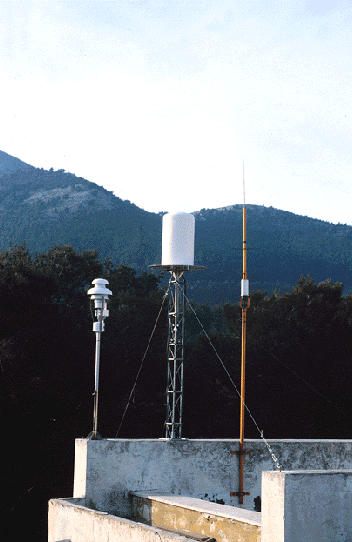
\includegraphics[width=0.7\textwidth]{DIOA}
    \caption{DORIS Beacon DIOA (Alcatel)}
    \label{fig:dioa}
  \end{subfigure}
  \begin{subfigure}[t]{0.45\textwidth}
    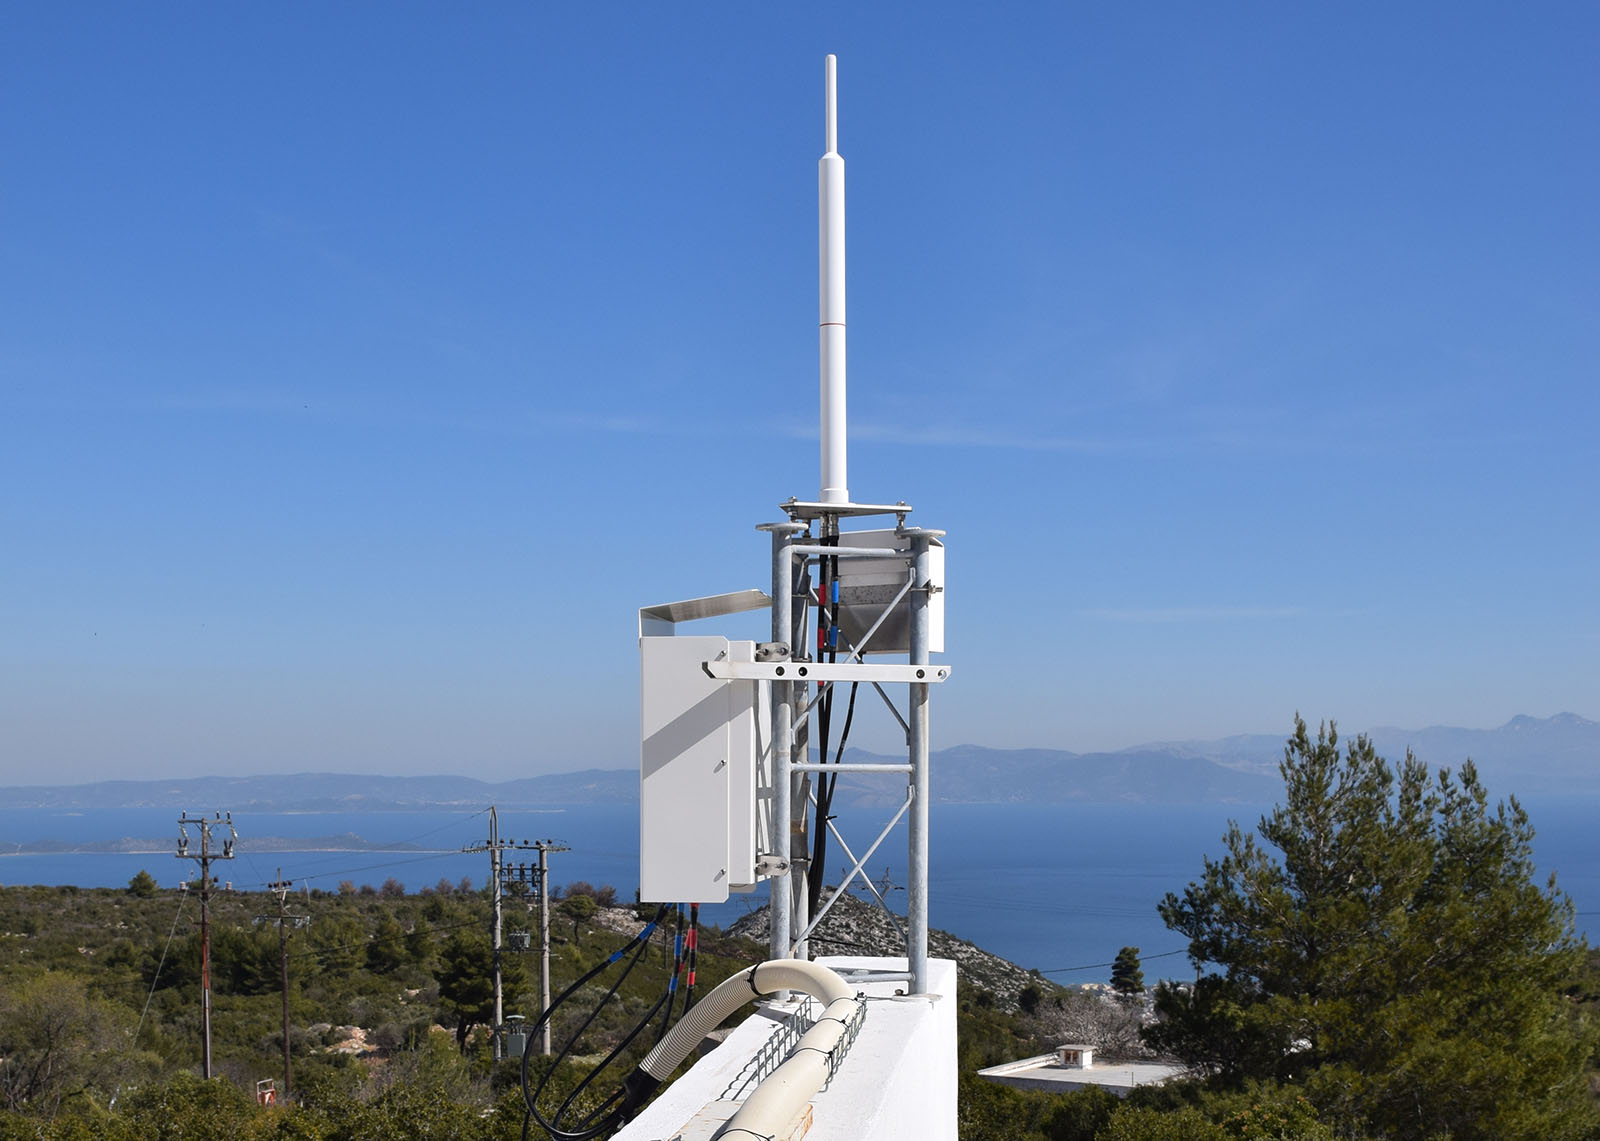
\includegraphics[width=1\textwidth]{DIOB_202103}
    \caption{DORIS Beacon DIOB (Starec)}
    \label{fig:diob}
  \end{subfigure}
  \caption{DORIS beacon hosted hosted at DSO facilities}
  \label{fig:dioa-and-diob}
\end{figure}
\end{frame}

\begin{frame}{}
\frametitle{Involvement in IDS \& Motivation}
  Since late 2021, DSO has decided to expand its involvement in the 
  DORIS community by developing its own, in-house processing software for 
  POD and positioning using the DORIS system.
  
  The software is designed and build \cul[blue!40]{from scratch}, adopting 
  recent developments in DORIS analysis and Satellite Geodesy.
\begin{itemize}[label=\textcolor{blue!40}{\textbullet}]
  \item expand out knowledge-base and expertise (research activity \& academic 
    services),
  \item follow and apply state-of-the-art technologies in Satellite Geodesy 
    and expand \& modernize our research activity,
  \item contribute to the DORIS/IDS community, and get involved ongoing/future 
    projects,
  \item fulfill PhD dissertation requirements
\end{itemize}
\end{frame}

\begin{frame}{}
\frametitle{Background}
Up to now, DSO has mainly be involved in precise GNSS positioning, primarily for 
monitoring the crustal dynamics of Greece, a region of complex tectonic \& 
volcanic background.

\begin{itemize}[label=\textcolor{blue!40}{\textbullet}]
  \item since 2015 we have established a monitoring platform using continuous 
    GNSS stations,
  \item daily, routine analysis of an extensive dataset,
  \item contribution to EUREF/EPN Densification (SINEX submission),
  \item time-series analysis (modeling of crustal dynamics)
\end{itemize}

All in all, we have extensive knowledge of GNSS analysis but a limited 
understanding of DORIS technology.
\end{frame}


\begin{frame}{}
\frametitle{Plan Outline}
Our goal is to develop a DORIS free and open-source analysis software for POD 
\& positioning.

We follow an incremental approach, integrating one component at a time. As a 
first step, we are targeting:
\begin{itemize}
  \item [\textcolor{blue!40}{\textbullet}] POD-only
  \begin{itemize}
    \item [\textcolor{blue!40}{\textbullet}] Jason-3 satellite
      \begin{itemize}
        \item [\textcolor{blue!40}{\textbullet}] adopt \& implement simple 
          models initially; gradually increase complexity (e.g. gravity 
          model)
       \end{itemize}
    \item [\textcolor{green!40}{\checkmark}] gradually incorporate more 
      satellites \ldots
  \end{itemize}
  \item [\textcolor{green!40}{\checkmark}] introduce positioning once POD is 
    acceptable
\end{itemize}

%Our intention is for the software to be \cul[blue!40]{free of charge }  
%and \cul[blue!40]{open-source}, so that the community can benefit as much as 
%possible.

%Separate distribution of binaries/scripts and libraries (building is cumbersome).
\end{frame}

\begin{frame}
  \frametitle{Design Considerations (1/2)}
  \begin{itemize}[label=\textcolor{blue!40}{\textbullet}]
    \item Core software development using the \textbf{C++} 
      programming language (exploiting its speed, robustness \& versatility)
    \item Various minor, peripheral parts developed using \textbf{Python}, 
      allowing development speed and ease of use (for developers \& users)
    \item Follow a \textbf{\emph{modular}} design pattern, with different 
      parts developed individually, serving specific needs, thus favoring 
      composability \& reusability
    \item Strive for \textbf{minimum dependencies}; when unavoidable, we 
      only use open-source software
    \item Developed in an ``\textbf{open}'' fashion, using public 
      repositories on \texttt{github}
  \end{itemize}
\end{frame}

\begin{frame}
  \frametitle{Design Considerations (2/2)}
  \begin{itemize}[label=\textcolor{blue!40}{\textbullet}]
    \item RINEX-only processing
    \item We try to follow, as close as possible, the latest IDS 
    recommendations published as 
    ``{\color{red!40}\emph{IDS Recommendations and suggestions for ITRF 2020 reprocessing}}''\footnote{\url{https://ids-doris.org/images/IDS_RecommendationsITRF2020_04.02.2020.pdf}} 
    or design for their easy adoption later on
    \item In general, consulting the extensive documentation on the IDS website 
    ``{\color{red!40}\emph{Documents for the data analysis}}''\footnote{\url{https://ids-doris.org/analysis-coordination/documents-related-to-data-analysis.html}}
    \item Handling of DORIS observations follows the approach outlined in \cite{lemoine-2016} 
      (range-rate)
    \item Estimation performed via Extended Kalman Filtering, \cite{tapley} (later 
      adopt a more sophisticated approach)
  \end{itemize}
\end{frame}

\begin{frame}
  \frametitle{Currently Implemented (Key Points)}
  \begin{itemize}[label=\textcolor{blue!40}{\textbullet}]
    \item orbit integration (using ``variational equations'')
    \item GPT3/VMF3 (\cite{Landskron2018}) tropospheric delay modeling
    \item quaternions for attitude (via published files)
    \item atmospheric drag force modeling, using the \emph{NRLMSISE00} model 
      \cite{nrlmsise00}
    \item strive for adherence to the latest IERS standards (\emph{IERS2010}, 
      \cite{iers2010})
    \item linear model for relative frequency offsets
    \item static gravity model (ICGEM-format)
    \item elevation-dependent weighting
    \item use of observation flags extracted from RINEX files (?)
  \end{itemize}
\end{frame}

\begin{frame}
  \frametitle{Flowchart}
  \begin{figure}
  \centering
  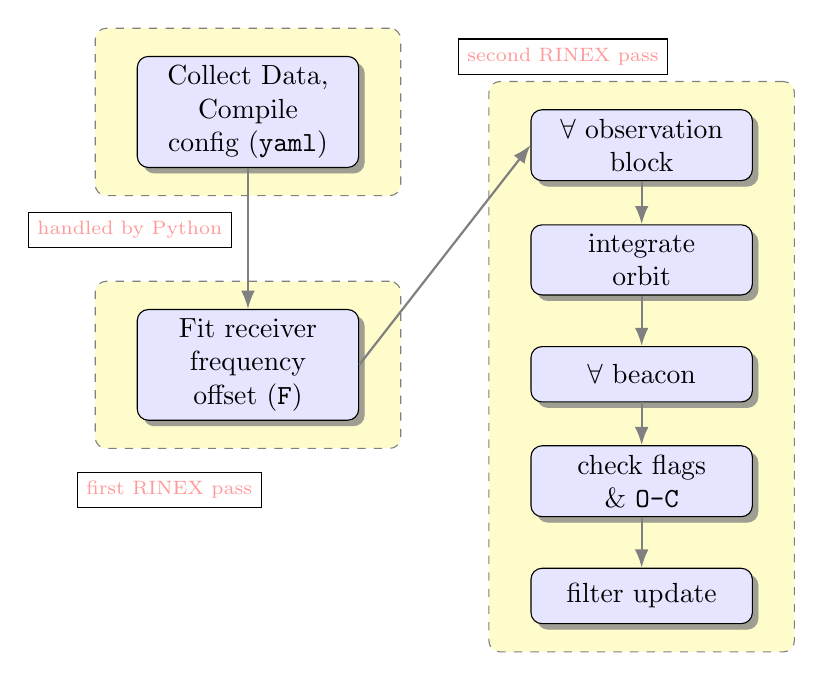
\begin{tikzpicture}
  % Draw diagram elements
  \path \etape{1}{Collect Data, Compile config (\texttt{yaml})};
  
  \path (p1.south)+(0.0, -2.5) \etape{2}{Fit receiver frequency offset (\texttt{F})};
  
  \path (p2.south)+(5.0, 3.5) \etape{3}{$\forall$ observation block};
  \path (p3.south)+(0.0,-1.0) \etape{4}{integrate orbit};
  \path (p4.south)+(0.0,-1.0) \etape{5}{$\forall$ beacon};
  \path (p5.south)+(0.0,-1.0) \etape{6}{check flags \& \texttt{O-C}};
  \path (p6.south)+(0.0,-1.0) \etape{7}{filter update};

  % Draw arrows between elements
  \path [line] (p1.south) -- node [above] {} (p2);
  \path [line] (p2.east) -- node [above] {} (p3.west);
  \path [line] (p3.south) -- node [above] {} (p4);
  \path [line] (p4.south) -- node [above] {} (p5);
  \path [line] (p5.south) -- node [above] {} (p6);
  \path [line] (p6.south) -- node [above] {} (p7);

  \begin{scope}[on background layer]
    \node (bk1) [back group] [fit=(p1)] {};
    \node (bk2) [back group] [fit=(p2)] {};
    \node (bk3) [back group] [fit=(p3) (p7)] {};
  %  \node [draw, thick, green!50!black, fill=green!75!black!25, rounded corners, fit=(p1), inner xsep=15pt, inner ysep=10pt] {};
  \end{scope}

  %\path (bk1.east)+(+6.0,0) node (ur1)[ur] {};
  %\transreceptor{bk1}{Python}{ur1}{east};
  \node[draw] at (-1.5,-1.5) {\scriptsize \textcolor{red!40}{handled by Python}};
  %\path [linepart] (#1.#4) -- node [above] {\scriptsize \textcolor{red!40}{#2}} (#3);}
  
  %\path (bk2.north)+(0.0,-4.0) node (ur2)[ur] {};
  %\transreceptor{bk2}{RINEX first pass}{ur2}{south};
  \node[draw] at (-1.0,-4.8) {\scriptsize \textcolor{red!40}{first RINEX pass}};
  \node[draw] at (4.0,+0.7) {\scriptsize \textcolor{red!40}{second RINEX pass}};

  \end{tikzpicture}
  \end{figure}
\end{frame}

\begin{frame}
  \frametitle{Thank you}
  \centering
  \textbf{Thank you for your attention!}
\end{frame}

\begin{frame}[allowframebreaks]
  \frametitle{References}
    \bibliography{doris}
\end{frame}

\appendix %do not count the following slides for the total number

\begin{frame}[plain]
  \frametitle{Not there yet \ldots}
\begin{figure}
  \centering
    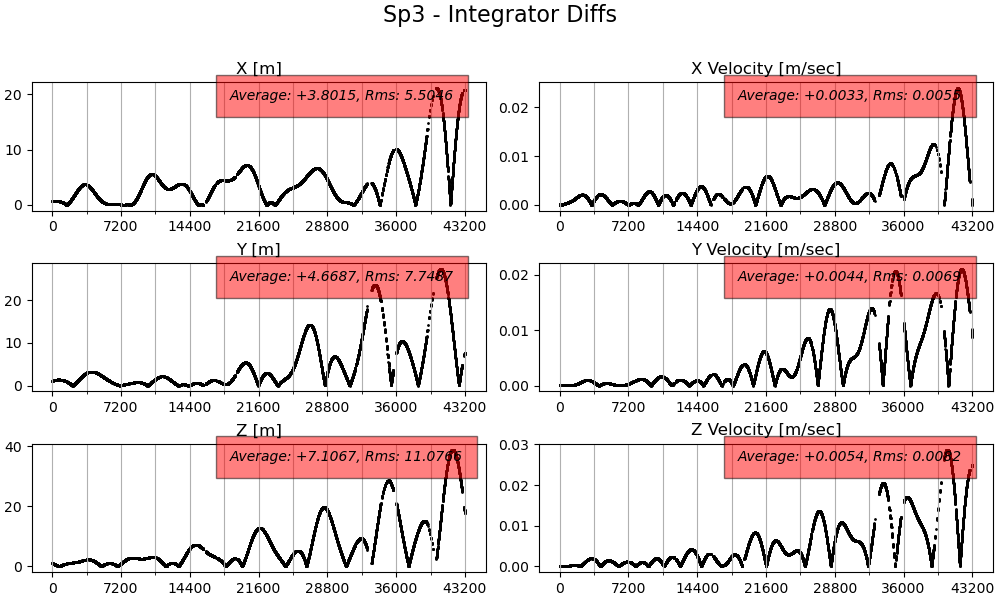
\includegraphics[width=0.8\textwidth]{neweop4}
    \caption{Conputed state Vs Sp3 results (Jason3, 02/01/2021)}
    \label{fig:sp3-vs-mine}
\end{figure}
\end{frame}

\end{document}
